\specialsection{Community}{}{black}{white}
\subsection{Forum}

\subsubsection*{Evolution of Community Discussion Platforms}
In the early days of the Processing project, community interactions predominantly took place on forums. These forums served as a primary channel for users to share experiences, discuss problems, and seek help. Notably, the forum discussions underwent significant transformations in terms of platforms over the years, as can be observed in Table \ref{table:forums}. \parencite{ProcessingForum}

\begin{table}[h]
    \raggedright
    \caption{Archival forums composition}
    \label{table:forums}
    \begin{tabular}{l l l c}
        \toprule
        Forum name & Years & URL \\
        \midrule
        Processing alpha forum & 2002-2005 & \href{https://forum.processing.org/alpha/}{forum.processing.org/alpha} \\
        Processing beta forum & 2005-2010 & \href{https://forum.processing.org/beta/}{forum.processing.org/beta}  \\
        Processing 1.0 forum & 2010-2013 & \href{https://forum.processing.org/one/}{forum.processing.org/one} \\
        Processing 2.0 and 3.0 forum & 2013-2018 & \href{https://forum.processing.org/two/}{forum.processing.org/two} \\
        Current processing forum & 2018 - now & \href{https://discourse.processing.org/}{discourse.processing.org} \\
        \bottomrule
    \end{tabular}
  \end{table}

This dynamic shift from one platform to another indicates an evolving user-base and a growing set of needs and tools that community members require for effective collaboration.

\begin{figure}
    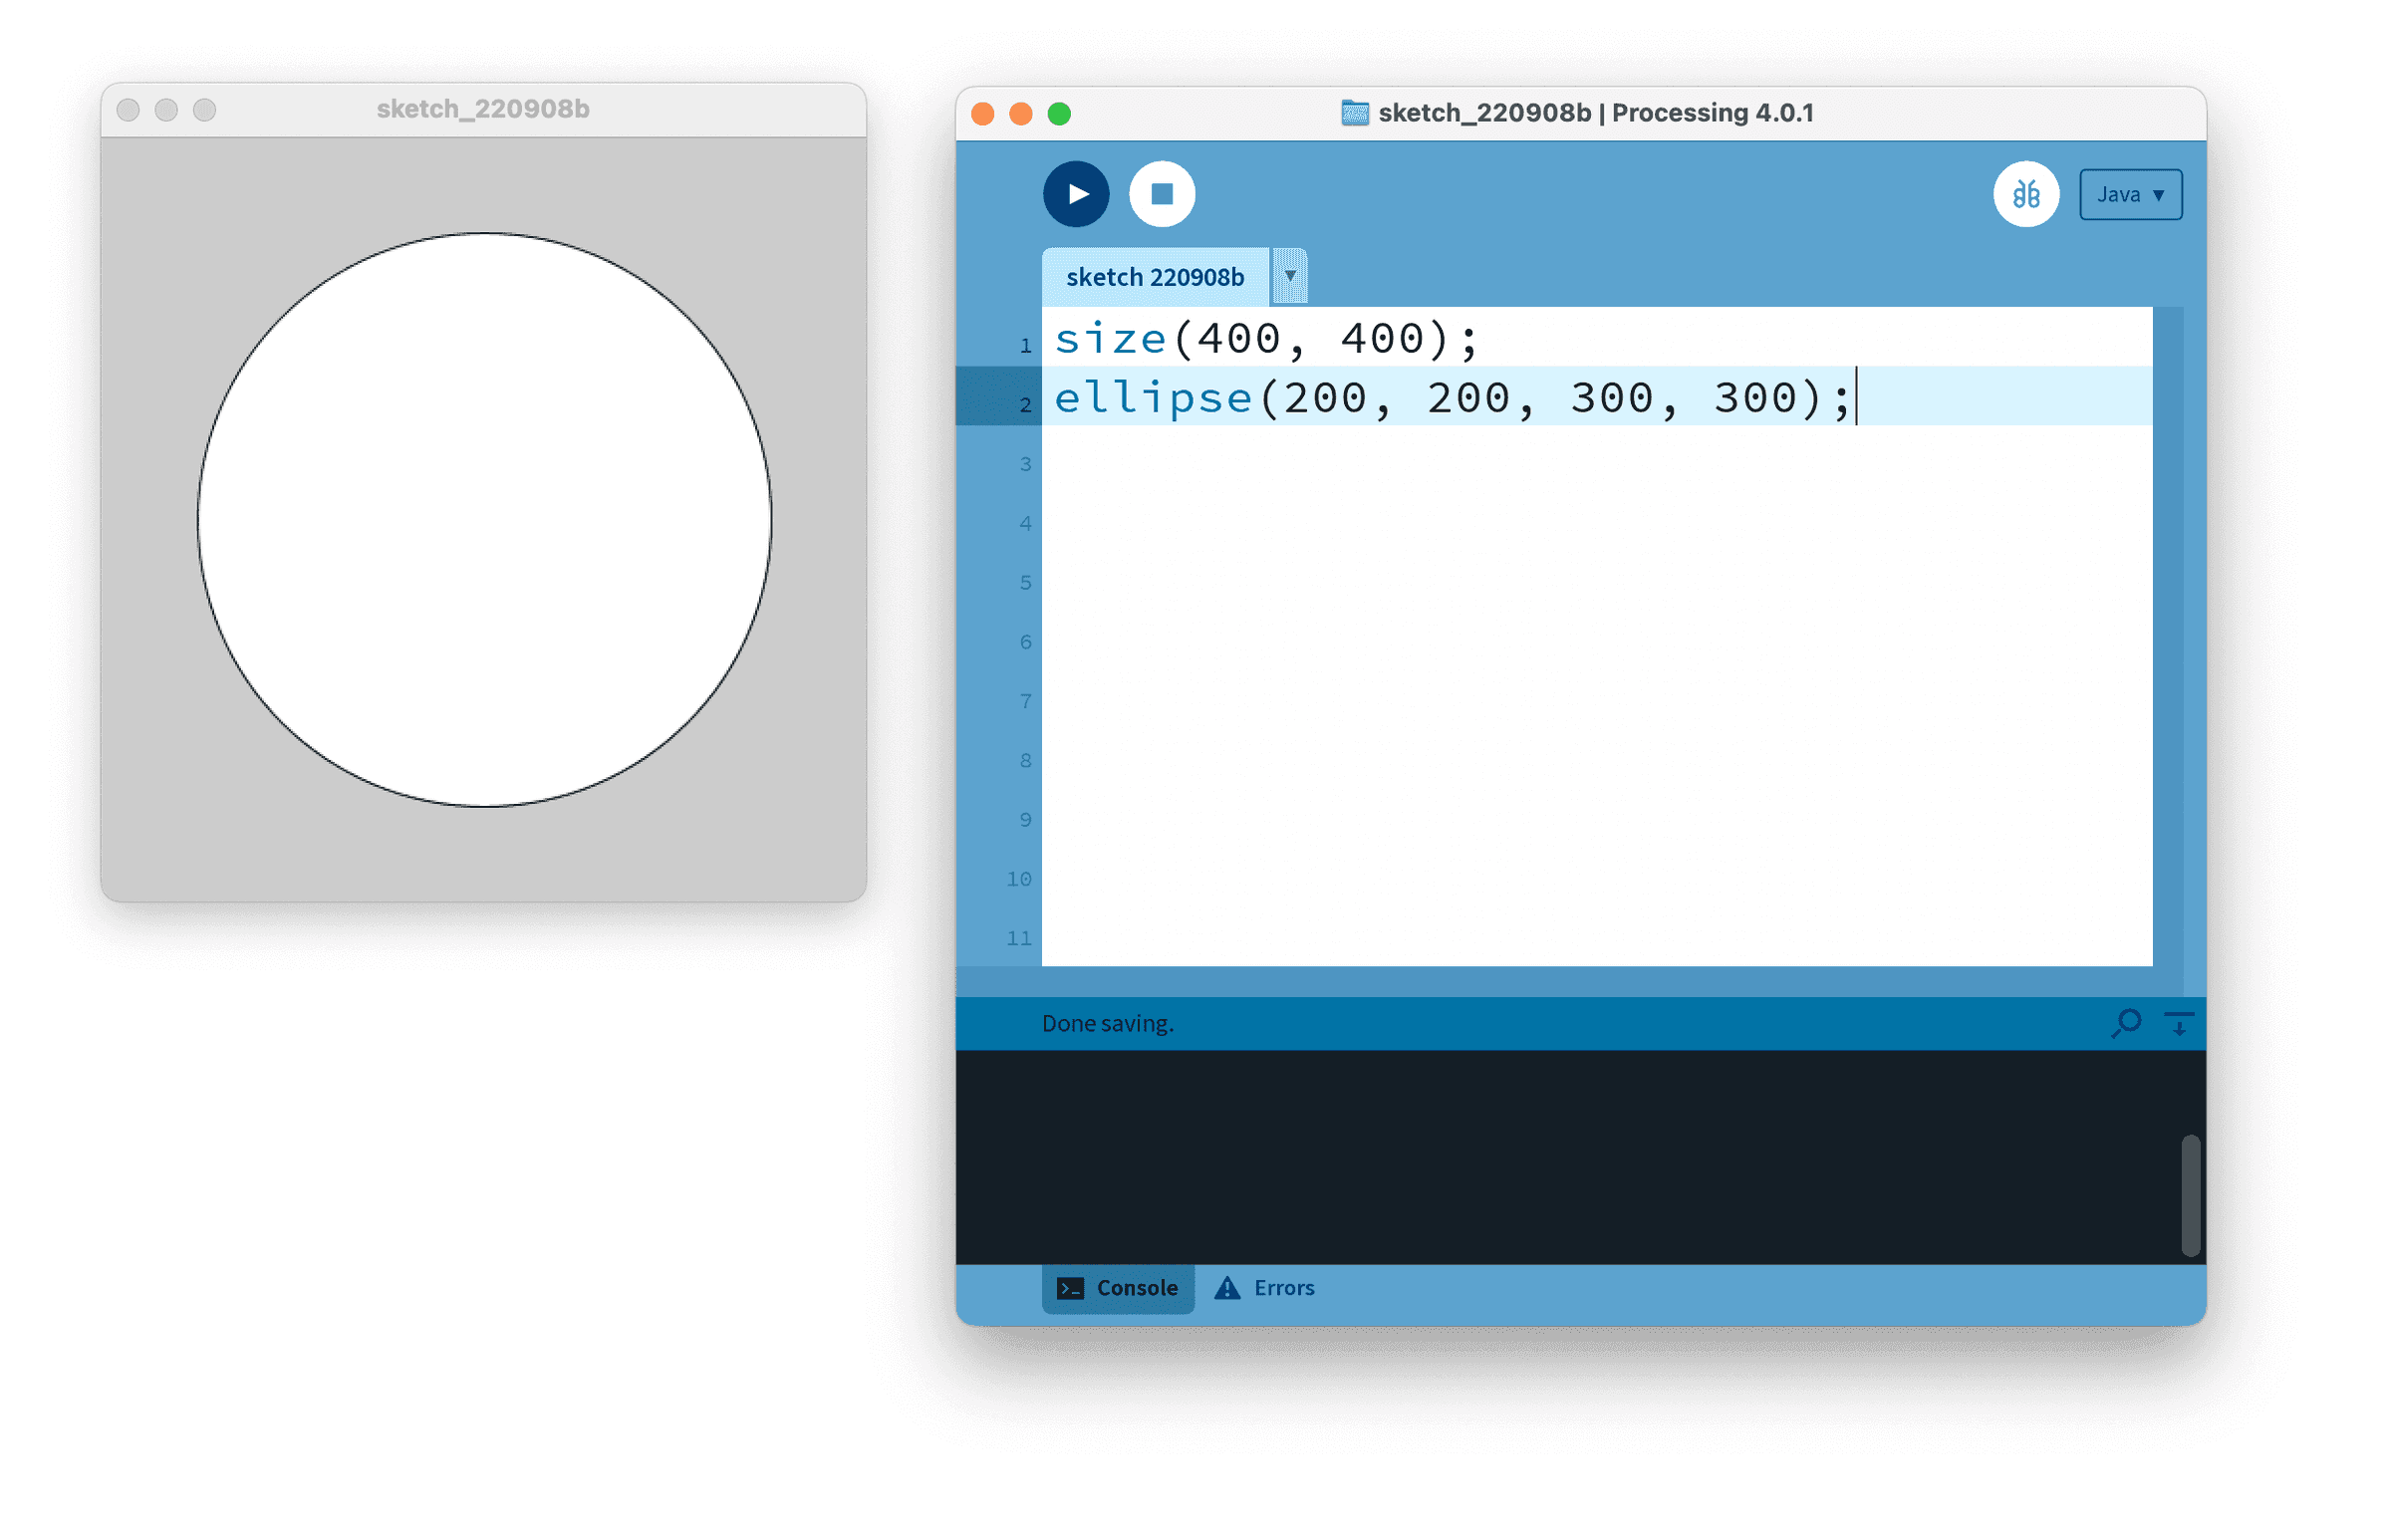
\includegraphics[width=1\textwidth]{images/processing_ide.png} 
    \caption{Processing IDE \parencite{reasProcessingIDE2015}}
    \label{fig:processing_ide_screenshot}
  \end{figure}
  

\subsection{Workshops}
\subsection{Libraries}
\subsection{Foundation}
